\chapter{Differential and Integral Calculus}

\vspace*{-1cm}
\begin{flushright}
\texttt{Step by step.}
\end{flushright}

\lettrine[nindent=0.35em,lhang=0.40,loversize=0.3]{I}{n a traditional}
introductory class of calculus, your teacher has probably started the discussion defining a function $x(t)$ and a pair of points $t_i$ and $t_f$. If you are a physicist, $x(t)$ was the trajectory defined by the position at time $t$. Within the finite interval $\Delta t = t_f-t_i$, the distance traveled is $\Delta x = x(t_f) - x(t_i)$. From these we can define the mean velocity within this interval as $\mean{v} = \Delta x/\Delta t$. Moreover, in the limit where $t_f$ and $t_i$ are infinitesimally close, we get the instantaneous velocity:

\begin{equation}
 v(t) = \dfrac{\partial}{\partial t} x(t) = \lim_{\Delta t \rightarrow 0} \dfrac{\Delta x}{\Delta t}.
\end{equation}

Using similar considerations your teacher has shown you that the integral is a sum of infinitesimal contributions:

\begin{equation}
 x(t) = x(0) + \int_0^t v(t') dt' = x(0) + \lim_{\Delta t' \rightarrow 0} \sum_{n=0}^{N} v\big(t'_n\big) \Delta t',
\end{equation}
where the sum runs over a discrete set labeled by the integer $0 \leq n \leq N$ that maps the time axes $0 \leq t'_n \leq t$.

If you remember all that, great! The main idea behind the numerical differential and integral calculus is to drop the infinitesimal limit and simply work with the finite differences. Of course this is too simple. It would be a crude approximation\footnote{Before continuing to the next section, please check Problem \ref{prob:SimpleIntegral} for some motivation.}. We can do better! But let's take it step by step... discrete steps.

\section{Interpolation / Discretization}

A numerical calculation usually require us to represent Real (continuous) axis, planes or volumes on the computer. This is impossible, right? Between 0.0 and 1.0 there's already $\infty$ numbers. We have to represent them in a discrete set, as introduced above.

The interpolation then deals with the unknown data in between discrete points. Let's start plotting \texttt{sin(x)} between $0 \leq x \leq 2\pi$ with a few points only.

\begin{example}{Discrete plot of \texttt{sin(x)}}
\begin{minted}{julia}
using PyPlot
x = linspace(0, 2pi, 7);
plot(x,  sin(x), "o")
plot(x,  sin(x), "-")
\end{minted}
\end{example}

In the example above, the first plot draws the circles, while the second draws the lines connecting them, equivalent to the green dots in Fig.~\ref{fig:interp}(a). The lines are a linear interpolation of the points. Try again with more or less points to see how it goes.

\begin{figure}[ht!]
 \centering
 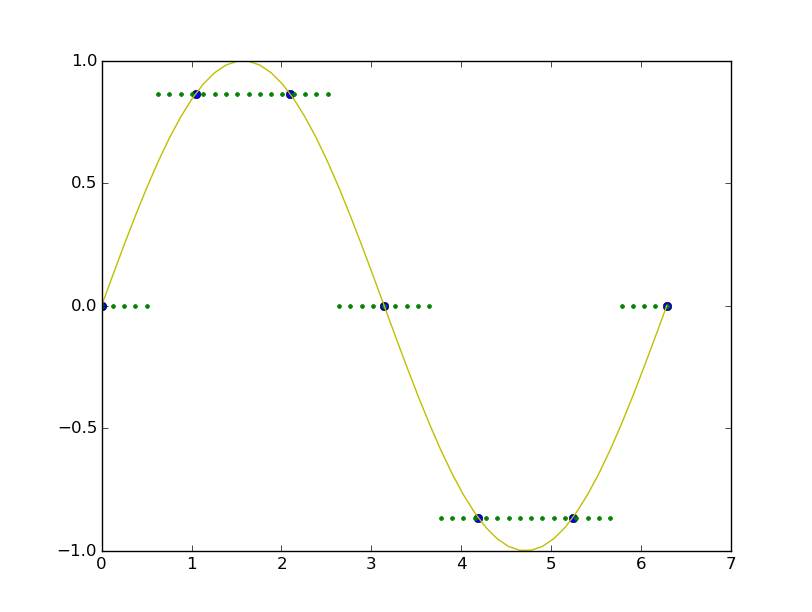
\includegraphics[width=0.32\textwidth,keepaspectratio=true]{./Interp0.png}
 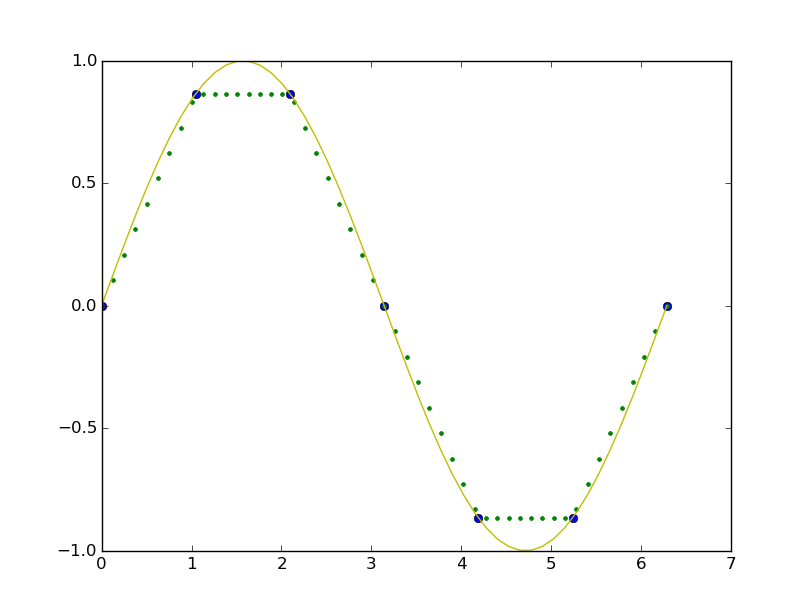
\includegraphics[width=0.32\textwidth,keepaspectratio=true]{./Interp1.png}
 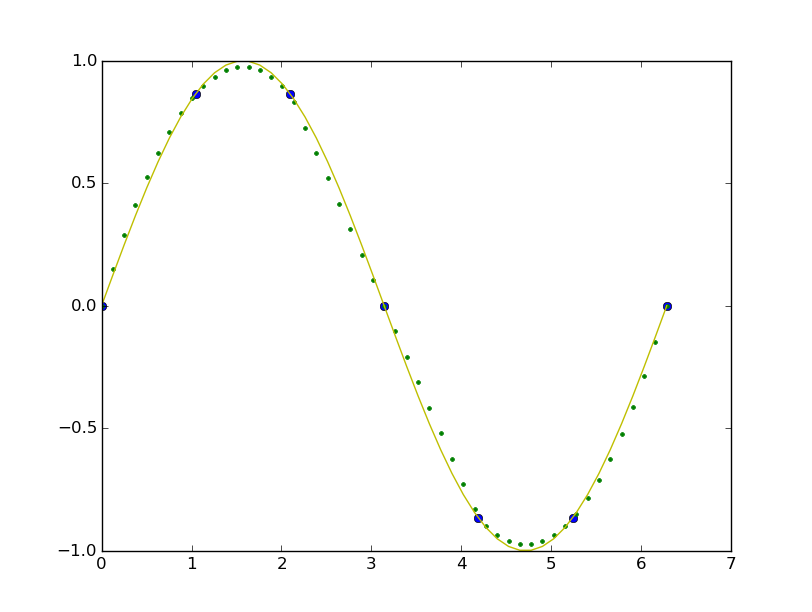
\includegraphics[width=0.32\textwidth,keepaspectratio=true]{./Interp2.png}
 \caption{Starting with the $\sin(x)$ defined at only 7 points (blue dotes), we calculate the (a) constant (rectangle) (b) linear (trapezoidal) and (c) quadratic interpolation points (green dots). In both panels the yellow lines show the exact $\sin(x)$ for comparison.}
 \label{fig:interp}
\end{figure}


\subsection*{Linear interpolation}

Say you have a finite set of points $\{x_n\}$ labeled by the integer $0 \leq n \leq N$, and you known the function $f(x)$ at these points. You may use the data from the example above with $f(x) = sin(x)$, or any other function of your choice.

Now, assume you want the value of the function at an general point $x$ that does not belong to your discrete set $\{x_n\}$, but lies within $x_a \leq x \leq x_b$. Here $b=a+1$ labeling consecutive points of the set. The most general expression for a linear interpolation connecting the points $\{x_a, f(x_a)\}$ and $\{x_b, f(x_b)\}$ is $\tilde{f}(x) = C_1 x+C_0$. We'll use the $\sim$ symbol to refer to the interpolated function. We want  $\tilde{f}(x)$ to match $f(x)$ at $x_a$ and $x_b$, therefore we have

\begin{align}
 \tilde{f}(x_a) &= C_1 x_a + C_0 = f(x_a),\\
 \tilde{f}(x_b) &= C_1 x_b + C_0 = f(x_b),
\end{align}
which defines a system of two equations and two unknowns ($C_1$ and $C_0$). This set of equations can be cast in a matrix form $M\cdot C = F$, where the matrix $M$, coefficient vector $C$ and function vector $F$ are show explicitly below:

\begin{equation}
 \begin{pmatrix}
  x_a & 1\\
  x_b & 1
 \end{pmatrix}
 \begin{pmatrix}
  C_1 \\ C_0
 \end{pmatrix}
 =
 \begin{pmatrix}
  f(x_a) \\ f(x_b)
 \end{pmatrix}.
\end{equation}

This equation can be easily solved as $C = M^{-1}\cdot F$. Evidently, you are able to express the result with paper \& pencil in this case. However, the matrix form makes it easy to generalize to higher order interpolation. The next example shows a code for linear interpolation, see Fig.~\ref{fig:interp}(a). In Problem \ref{prob:interpolation} I ask you to generalize this code for a quadratic interpolation that should result in Fig.~\ref{fig:interp}(b). 

As you can see, the quadratic interpolation is already very close to the exact $\sin(x)$ function. The interpolations usually work well because we are almost always dealing with analytical functions, smooth functions. Complicated functions will probably require advanced methods. For instance, functions with singularities.

\begin{example}{Code for Linear Interpolation}
\label{ex:quadraticinterp}
\begin{minted}{julia}
using PyPlot

xlst = linspace(0, 2pi, 7); # create data for the example
flst = sin(xlst);

# receives number of points n (odd) to interpolate
# and the original data via x and f
function interp1(n, x, f)
    xnew = linspace(x[1], x[end], n); # creates new axes
    fnew = zeros(n); # and initialize new data as zero

    i = 1; # label new sites
    for j=1:(length(x)-1) # runs over old sites
        xa = x[j]; # known points
        xb = x[j+1];
        fa = f[j]; # known data
        fb = f[j+1];
        
        # matrix form to find the coefficients
        M = [xa 1.0; xb 1.0];
        C1, C0 = inv(M)*[fa; fb];

        # calculate the new data within every two points interval
        while i <= n && xnew[i] <= xb
            fnew[i] = C1*xnew[i] + C0;
            i += 1;
        end
    end
    return xnew, fnew; # return interpolated data
end

# calls function to interpolate
xnew, fnew = interp1(51, xlst, flst);

# plot old data, new data, and exact function
plot(xlst, flst, "o");
plot(xnew, fnew, "g.");
plot(xnew, sin(xnew), "y-");
\end{minted}
\end{example}



\section{Numerical Integration - Quadratures}

Common numerical integration schemes rely on simple interpolations (Newton–Cotes rules). Let's discuss these methods first. Later we give an overview of adaptive integration schemes, which is natively implemented in Julia as the function \texttt{quadgk}, and more sophisticated implementations for multi-dimensional integrals can be found on the \texttt{Cubature} package. We finish this section discussing the Monte Carlo integration technique.

\subsection{Polynomial Interpolations}

We have briefly discussed polynomial interpolations in the previous section. Now we'll use different interpolations to define common quadrature schemes. To establish a notation, we'll refer to the discrete points as $x_n$, where the integer $n$ labels the points as in Fig. ?. We'll assume that the set of points $\{x_n\}$ is equally spaced, so we can define a constant step $\Delta x = x_{n+1}-x_{n}$.

\subsection*{Rectangle rule}

The simplest quadrature method is the \textit{rectangle rule}. Here the function is assumed to be constant and equal to $f(x_n)$ within the interval $x_n-\Delta x/2 \leq x \leq x_n+\Delta x/2$. The interpolation resulting from this rule can be seen in Fig.~\ref{fig:interp}(a). Consequently, the integral over this range is

\begin{equation}
 \int_{x_n-\frac{\Delta x}{2}}^{x_n+\frac{\Delta x}{2}} f(x) dx \approx f(x_n) \Delta x + \mathcal{O}(\Delta x).
\end{equation}


\subsection*{Trapezoidal rule}

The trapezoidal rule uses the linear interpolation shown in Fig.~\ref{fig:interp}(b). It is easy to see (Prob.~\ref{prob:quadrature}) that this leads to 

\begin{equation}
 \int_{x_n}^{x_{n+1}} f(x) dx \approx \dfrac{f(x_{n+1}) + f(x_n)}{2}\Delta x + \mathcal{O}(\Delta x^2).
\end{equation}

\subsection*{Simpson's rule}

If we use the parabolic interpolation, we get Simpson's rule:

\begin{equation}
 \int_{x_n}^{x_{n+2}} f(x) dx \approx \Big[f(x_n) + 4 f(x_{n+1}) + f(x_{n+2})\Big] \dfrac{\Delta x}{3} + \mathcal{O}(\Delta x^4).
\end{equation}

From Fig.~\ref{fig:interp} one can already expect that the Simpson's rule to give better results and the rectangular or trapezoidal rules.

\subsection*{General remarks on the rules above}

Note that the trapezoidal rule is defined over a range set by two consecutive points, while the Simpson's rule runs over three points, from $x_n$ to $x_{n+2}$. As a consequence the Simpson's rule can only be used if you have an odd number of known points.

Higher order polynomials leads to more precise quadrature rules. Cubic interpolation leads to the Simpson's $3/8$ rule, which uses 4 points. For polynomial interpolations of degree 4 we get Boole's rule, which uses 5 points.

In the next example I assume we have a discrete set of points given by \texttt{xlst} and \texttt{flst} that correspond to the output of some previous calculation. The function \texttt{trapezoidal} is then used to integrate the function. Problem \ref{prob:SimpleIntegral} asks you to implement other rules. Try to change the number of points in the example, as well as other more complicated functions.

\begin{example}{Numerical quadrature of a discrete function}
\label{ex:numericalquadrature}
\begin{minted}{julia}
# receives two vectors for the axis x and function f
function trapezoidal(x, f)
   delta = x[2]-x[1]; # assuming constant step
   res = 0.0; # initializes the sum
   for n=1:(length(x)-1)
       res += 0.5*(f[n+1]+f[n])*delta; # traditional rule
   end
   return res; # returns the result
end

# create data for the example
xlst = linspace(0, 2pi, 7); # x axis
flst = sin(xlst); # discretized function f(x)

trapezoidal(xlst, flst) # calls the function and shows the result
\end{minted}
\end{example}

We may also need to integrate an exact function $f(x)$. This is done in the next example. Now the \texttt{trapezoildal} function receives the function to be integrated, the limits of integration, and the number of points to consider. Here the function is never written as a vector. Instead, it is calculated as needed. This will be more efficient for integration with a large number of points, as it doesn't store the function as the vector \texttt{flst} as above.

\begin{example}{Numerical quadrature of a function f(x)}
\label{ex:numericalquadrature2}
\begin{minted}{julia}
# receives the function g(x) to be integraded
# from x=a to x=b with n points
function trapezoildal(g, a, b, n)
   dx = (b-a)/(n-1.0);
   xi(i) = a + (i-1.0)*dx;
   res = 0.0;	
   for i=1:(n-1)
      res += 0.5*(g(xi(i+1))+g(xi(i)))*dx
   end
   return res;
end

f(x) = sin(x); # chosen function

trapezoildal(f, 0, pi, 3) # test with 3 points

trapezoildal(f, 0, pi, 20) # 20 points

trapezoildal(f, 0, pi, 100) # 100 points
\end{minted}
\end{example}

Note that these examples illustrate two distinct cases. In Example \ref{ex:numericalquadrature} we assume that some previous calculation has given us the axis discretized into the vector \texttt{xlst} as well as the function \texttt{f(x)} calculated at these points and stored in the vector \texttt{flst}. This means that we are assuming that we don't have direct access to an exact function \texttt{f(x)}. 

Example \ref{ex:numericalquadrature2} presents the opposite case. Here we do have access to the exact function \texttt{f(x)}. In this case one may use more sophisticated quadrature schemes. We present some of them in the next section.

\subsection{Adaptive and multi-dimensional integration}

Julia already has a native quadrature code implemented (\texttt{quadgk}). It uses an adaptive Gauss-Kronrod integration technique. Since this is an introductory class, I will not go into details of this method\footnote{Those who are interested in mode details, please check the Wikipedia page for Adaptive quadrature and references within: \url{https://en.wikipedia.org/wiki/Adaptive_quadrature}}. 

But to get an idea of how the code works, imagine you have two quadrature of different order implemented, say the trapezoidal and Simpson's rules, and you want to integrate \texttt{f(x)} from \texttt{x=a} to \texttt{x=b}. First you split your integration into subintervals, say from \texttt{x=a} to \texttt{x=c}, and from \texttt{x=c} to \texttt{x=b}, \textit{i.e.}

\begin{equation}
 \int_a^b f(x) dx = \int_a^c f(x) dx + \int_c^b f(x) dx.
\end{equation}
Then you evaluate each integral on the right hand side independently. You can estimate the error of each subinterval comparing the result of the  trapezoidal and Simpson's rules. If the error of a subinterval is too big, you split it into a new pair of subintervals and repeat the test until you converge to the desired error.

An efficient implementation of such methods can be difficult, and I leave it as a challenge for the experienced programmers in Problem \ref{prob:adaptive}.

Luckily, Julia has already the function \texttt{quadgk}. Check its documentation for details on the parameters. The next example shows a basic usage.

\begin{example}{Numerical quadrature with \texttt{quadgk}}
\label{ex:quadgk}
\begin{minted}[mathescape]{julia}
# let's start with the same function from the previous example
f(x) = sin(x);
# quadgk receives the function and the limits of integration
quadgk(f, 0, pi)

# you may also try functions with integrable singularities...
f(x) = 1/sqrt(x);
quadgk(f, 0, 16) # exact result is 8

# and integrate all the way to infinity (Inf)
f(x) = exp(-(x^2)/2)/sqrt(2);
res = quadgk(f, -Inf, Inf) # exact result is $\sqrt{\pi}$
pi-res[1]^2 # compare to $\pi$ to check the error
\end{minted}
\end{example}

For more advanced routines and multi-dimensional integration, please check Julia's \texttt{Cubature} package\footnote{Cubature package: \url{https://github.com/stevengj/Cubature.jl}}.

\subsection{Monte Carlo integration}

While the previous methods integrate functions sampling them along a regular grid, the Monte Carlo integration scheme samples the integration interval using random numbers. We have used this method already to calculate $\pi$ back in Problem \ref{prob:pi}, which can be recast as a two-dimensional integral:

\begin{equation}
 f(x,y) =
   \begin{cases} 
   4  & \text{if } x^2+y^2 \leq 1, \\
   0  & \text{otherwise,}
  \end{cases}
\end{equation}

\begin{equation}
 \pi = \int_\Omega f(x,y) dx dy,
\end{equation}
where the integration area $\Omega$ is set by the ranges $0 \leq x \leq 1$ and $0 \leq y \leq 1$.

The Monte Carlo implementation of this integral reads

\begin{equation}
 R_N = \dfrac{1}{N} \sum_{i=1}^N f(x_i, y_i).
\end{equation}

The next example shows an implementation of this integral

\begin{example}{Monte Carlo integral to calculate $\pi$}
\label{ex:montecarlopi}
\begin{minted}[mathescape]{julia}
function Rn(f, n) # Monte Carlo integration of f(x,y)
   res=0.0;
   for i=1:n
      res += f(rand(), rand());
   end
   return res/n;
end

# define the function using the ternary operator
f(x,y) = (x^2+y^2 <= 1.0)?4.0:0.0;

Rn(f, 10) # run the integral with 10 points
Rn(f, 1000) # run the integral with 100 points
\end{minted}
\end{example}

The main advantage of the Monte Carlo integral is that its error decays with $1/\sqrt(n)$ independently of the dimensions of the integral. Therefore this method becomes very interesting for high-dimensional integrals.

\section{Numerical Derivatives}

At the beginning of this Chapter, our overview of the numerical calculus introduced the idea of a numerical derivative simply as dropping the infinitesimal limit on the definition of a derivative. Indeed this leads to a familiar expression:

\begin{equation}
 \dfrac{\partial f(x)}{\partial x} = \lim_{\Delta x \rightarrow 0} \dfrac{f(x+\Delta x) - f(x)}{\Delta x} \approx \dfrac{f(x+\Delta x) - f(x)}{\Delta x}.
\end{equation}
As far as $\Delta x$ is small, this should give us a good estimate of the derivative. This formula is actually known as the \textbf{forward} derivative, as it gives the derivative of $f(x)$ at $x$ using two points: $x$ itself, and the one step forward $x+\Delta x$.

\subsection{Finite differences and Taylor series}

The finite differences scheme is the most common method for numerical differentiation. Its arises from the Taylor expansion of a function $f(x)$:

\begin{equation}
 f(x_i+h) = f(x_i) + h \left.\dfrac{\partial f}{\partial x}\right|_{x_i} + \dfrac{h^2}{2!}\left.\dfrac{\partial^2 f}{\partial x^2}\right|_{x_i}
 +\dfrac{h^3}{3!}\left.\dfrac{\partial^3 f}{\partial x^3}\right|_{x_i} + \cdots
 \label{eq:fwdTaylor}
\end{equation}
Here $x_i$ is an arbitrary point of our discrete grid labeled by the integer $i$, and $h$ is the step size between discrete points.

Let's use the Taylor expansion to get the $1^{st}$ and $2^{nd}$ derivatives of $f(x)$ using two or three points of the discrete axis $x \rightarrow x_i$.

\subsection*{Forward $1^{st}$ derivative}

If we truncate the Taylor expansion on the $h^2$ term, we can rearrange the remaining terms to read:

\begin{equation}
 \left.\dfrac{\partial f}{\partial x}\right|_{x_i} \approx \dfrac{f(x_i+h) - f(x_i)}{h} + \mathcal{O}(h)
\end{equation}

\subsection*{Backward $1^{st}$ derivative}

Another choice is to start with the Taylor expansion for a negative step

\begin{equation}
 f(x_i-h) = f(x_i) - h \left.\dfrac{\partial f}{\partial x}\right|_{x_i} + \dfrac{h^2}{2!}\left.\dfrac{\partial^2 f}{\partial x^2}\right|_{x_i}
 -\dfrac{h^3}{3!}\left.\dfrac{\partial^3 f}{\partial x^3}\right|_{x_i} + \cdots
 \label{eq:bwdTaylor}
\end{equation}
and once again truncate the expansion on the $h^2$ term to get

\begin{equation}
 \left.\dfrac{\partial f}{\partial x}\right|_{x_i} \approx \dfrac{f(x_i) - f(x_i-h)}{h} + \mathcal{O}(h)
\end{equation}

\subsection*{Symmetric (or central) $1^{st}$ derivative}

Subtracting Eq.~\eqref{eq:fwdTaylor} from Eq.~\eqref{eq:bwdTaylor} we eliminate the $h^2$ term

\begin{equation}
 f(x_i+h) - f(x_i-h) = 2h \left.\dfrac{\partial f}{\partial x}\right|_{x_i} + 2\dfrac{h^3}{3!}\left.\dfrac{\partial^3 f}{\partial x^3}\right|_{x_i} + \cdots
\end{equation}
and now we can truncate the sum on the $h^3$ term to get

\begin{equation}
 \left.\dfrac{\partial f}{\partial x}\right|_{x_i} \approx \dfrac{f(x_i+h) - f(x_i-h)}{2h} + \mathcal{O}(h^2)
\end{equation}


\subsection*{Symmetric (or central) $2^{nd}$ derivative}

This time let's sum Eqs.~\eqref{eq:fwdTaylor} and \eqref{eq:bwdTaylor} to eliminate the first derivative:

\begin{equation}
 f(x_i+h) + f(x_i-h) = 2f(x_i) + h^2\left.\dfrac{\partial^2 f}{\partial x^2}\right|_{x_i} + \cdots
\end{equation}
Rearranging the expansion truncated on the $h^4$ term give us

\begin{equation}
 \left.\dfrac{\partial^2 f}{\partial x^2}\right|_{x_i} \approx \dfrac{f(x_i+h) - 2f(x_i) + f(x_i-h)}{h^2} + \mathcal{O}(h^2)
\end{equation}

Run the next example to get a plot comparing the first derivatives with the exact result. Try changing the step size from \texttt{h=pi/5} to \texttt{pi/50} and \texttt{pi/500}.

\begin{example}{Derivative using finite differences}
\label{ex:finitedifferences}
\begin{minted}[mathescape]{julia}
# simple implementation of the finite differences
diff1_forward(f, x, h) = (f(x+h)-f(x))/h;
diff1_backward(f, x, h) = (f(x)-f(x-h))/h;
diff1_symmetric(f, x, h) = (f(x+h)-f(x-h))/(2h);

f(x) = sin(x); # chosen function to test

xgrid = 0:(pi/50):pi; # discrete x axis
h = pi/5; # step for the derivatives

# using comprehensions to calculate the derivatives along xgrid
fwd = [diff1_forward(f, x, h) for x=xgrid]
bwd = [diff1_backward(f, x, h) for x=xgrid]
sym = [diff1_symmetric(f, x, h) for x=xgrid]

# plot the exact result and the approximate derivatives for comparison
clf();
plot(xgrid, cos(xgrid); label="cos(x)")
plot(xgrid, fwd; label="forward")
plot(xgrid, bwd; label="backward")
plot(xgrid, sym; label="symmetric")
legend()
\end{minted}
\end{example}

In the example above we are assuming that we have access to the exact function $f(x)$ at any point. This is similar to what we saw in Example \ref{ex:numericalquadrature2}. What happens if we consider a situation similar to the one in Example \ref{ex:numericalquadrature}? There we assume that we only known the function $f(x)$ via the discrete points set by \texttt{xlst} and \texttt{flst}. Check \mbox{Problem \ref{prob:finitediff2}.}

\subsection{Matrix Representation}
\label{sec:matrixrepresentation}

Sometimes it is useful to represent the derivatives in matrix forms, such that it becomes an operator. Say that we have a discrete $x$ axis labeled by $x_i$ for $1 \leq i \leq N$, and a function defined at these points by $f_i = f(x_i)$. These are exactly the \texttt{xlst} and \texttt{flst} vectors from the previous Examples of this Chapter. Let's assume that $f_i = 0$ for $i \leq 0$ and $i \geq N+1$. Let's write the expressions for the symmetric finite differences derivative $f'_i = \left.\frac{\partial f(x)}{\partial x}\right|_{x_i}$ at each point $x_i$:

\begin{align}
 \text{for i=1, }\quad f'_1 &= \dfrac{f_2-0}{2h},\\
 \text{    i=2, }\quad f'_2 &= \dfrac{f_3-f_1}{2h},\\
 \text{    i=3, }\quad f'_3 &= \dfrac{f_4-f_2}{2h},\\
 \text{    i=4, }\quad f'_4 &= \dfrac{f_5-f_3}{2h},\\
          \cdots \quad f'_i &= \dfrac{f_{i+1}-f_{i-1}}{2h},\\
 \text{  i=N-1, }\quad f'_{N-1} &= \dfrac{f_N-f_{N-2}}{2h},\\
 \text{  i=N,   }\quad f'_{N} &= \dfrac{0-f_{N-1}}{2h}.
\end{align}
The zero in the first and last lines refer to $f_0 = 0$ and $f_{N+1} = 0$, respectively.

The set of equations above can be put in a matrix form as

\begin{equation}
 \begin{pmatrix}
  f'_1 \\f'_2 \\ f'_3 \\ f'_4 \\ \cdots \\ f'_i \\ \cdots \\ f'_{N-1} \\ f'_N
 \end{pmatrix}
 = \dfrac{1}{2h}
\begin{pmatrix} 
 0 & 1 & 0 & 0 & 0 & 0 & 0 & 0 & 0\\
 -1 & 0 & 1 & 0 & 0 & 0 & 0 & 0 & 0\\
 0 & -1 & 0 & 1 & 0 & 0 & 0 & 0 & 0\\
 0 & 0 & -1 & 0 & 1 & 0 & 0 & 0 & 0\\
 0 & 0 & 0 & -1 & 0 & 1 & 0 & 0 & 0\\
 0 & 0 & 0 & 0 & -1 & 0 & 1 & 0 & 0\\
 0 & 0 & 0 & 0 & 0 & -1 & 0 & 1 & 0\\
 0 & 0 & 0 & 0 & 0 & 0 & -1 & 0 & 1\\
 0 & 0 & 0 & 0 & 0 & 0 & 0 & -1 & 0
\end{pmatrix}
\begin{pmatrix}
  f_1 \\f_2 \\ f_3 \\ f_4 \\ \cdots \\ f_i \\ \cdots \\ f_{N-1} \\ f_N
\end{pmatrix}
\end{equation}

In Julia this matrix can be implemented using the \texttt{diagm} function:

\begin{example}{Matrix representation of the first derivative}
\label{ex:matrix}
\begin{minted}[mathescape]{julia}
x = linspace(-10, 10, 101); # discrete x axis
f = exp(-(x.^2)/2.0); # function sampled at x

n = length(x); # number of points
h = x[2] - x[1]; # step size

matdiff = (diagm(ones(n-1), 1) - diagm(ones(n-1), -1))/(2h);

# calculates the derivative of f as a product of matrix and vector
dfdx = matdiff*f; 

plot(x, dfdx);
\end{minted}
\end{example}

\subsection{Derivatives via convolution with a kernel}

A one-dimensional (1D) discrete convolution of the vectors \texttt{f} and \texttt{g} read

\begin{equation}
 (g \ast f)[n] = \sum_{m=1}^N g[m]f[n+N-1-m],
\end{equation}
where the index of our arrays $g[m]$ and $f[m]$ start at 1 and $N$ is the length of the array $g$.



Let's refer to the vector \texttt{g} as the kernel, and \texttt{f} as our function. If the kernel is \mbox{$g = \frac{1}{2h}(1, 0, -1)$}, the convolution above becomes

\begin{equation}
 (g \ast f)[n] = \dfrac{1}{2h}\Big(f[n+1] - f[n-1]\Big),
\end{equation}
which is exactly our definition of the symmetric first derivative. 

In Julia we can use the \texttt{conv} function for 1D convolutions and the \texttt{conv2} function for two-dimensional (2D) convolutions. The next example can be compared with the previous one. Note that after the convolution we remove end points to keep \texttt{dfdx} with the same size of \texttt{x}.

\begin{example}{Derivatives via convolution with a kernel 1D}
\label{ex:conv}
\begin{minted}[mathescape]{julia}
x = linspace(-10, 10, 101); # discrete x axis
f = exp(-(x.^2)/2.0); # function sampled at x

n = length(x); # number of points
h = x[2] - x[1]; # step size

# kernel for the symmetric first derivative 1D
kernel = [1.0; 0.0; -1.0]/(2h);

dfdx = conv(kernel, f); # convolution
dfdx = dfdx[2:end-1]; # remove end points

plot(x, dfdx);
\end{minted}
\end{example}

In 2D the kernel becomes a matrix. For instance, the kernel for $\frac{\partial^2}{\partial x \partial y}$ represented by the symmetric differences with step sizes $h_x$ and $h_y$ in each direction is

\begin{equation}
 g = \dfrac{1}{4 h_x h_y}
 \begin{pmatrix}
  0 & 1 & 0 \\
  1 & 0 & -1 \\
  0 & -1 & 0
 \end{pmatrix}.
\end{equation}

\begin{example}{Derivatives via convolution with a kernel 2D}
\label{ex:conv2}
\begin{minted}[mathescape]{julia}
# x and y axes
# transpose y to get matrix mesh for f later on
x = linspace(-5, 5, 101);
y = transpose(linspace(-5, 5, 101));
hx = x[2]-x[1]; # step sizes
hy = y[2]-y[1];

# 2D function as a matrix (lines are x, columns are y)
f = exp(-(x.^2)/2).*exp(-(y.^2)/2);

# 2D kernel for $\frac{\partial^2}{\partial x \partial y}$
kernel = (1.0/(4*hx*hy))*[0.0 1.0 0.0; 1.0 0.0 -1.0; 0.0 -1.0 0.0];

df = conv2(kernel, f); # 2D convolution
df = df[2:end-1, 2:end-1]; # remove end points

surf(x, y', df) # surface plot
# requires y to be transposed back into a column vector
\end{minted}
\end{example}


\subsection{Other methods, Julia commands and packages for derivatives}

Later on we'll see how to take derivatives using the properties of Fourier transforms. This will be useful to solve differential equations, for instance with the split-operator or split-step methods.

Julia has a native command for the first order derivatives: \texttt{gradient}. This command uses the forward rule to evaluate the derivative at the first point, the backward rule at the last point, and the symmetric rule at the internal points.

There exists also packages, like the \texttt{ForwardDiff}\footnote{ForwardDiff package: \url{https://github.com/JuliaDiff/ForwardDiff.jl}}. However there's a warning on the webpage of \texttt{ForwardDiff} and at this moment I'm not familiarized with the issues they are facing.

\section{Problems}

\begin{problem}{Checking the simplest numerical integration}
 \label{prob:SimpleIntegral}

 Consider the functions $f(x) = \sin(x)$, $g(x) = \cos(x)$, and $h(x) = e^x$.
 
 \textbf{a)} What is the exact result for the integration of $f(x)$ and $g(x)$ on the interval $0 \leq x \leq 2\pi$? Try also the interval $0 \leq x \leq \pi$. What about the integration of $h(x)$ over $0 \leq x \leq 1$?
 
 \textbf{b)} Try to numerically integrate these functions as initially described at the introduction of this chapter. Simply dropping the infinitesimal limit. Compare the deviation from the exact result as a function of the number of points used in the integration in a log-plot. Useful Julia commands: \texttt{linspace}, \texttt{sum}.
 
 \textbf{c)} Complement item \textbf{(b)} as you learn new methods: compare the precision of different methods (trapezoidal, Simpson's, Boole's, Monte Carlo, ...) as a function of the number of points being used.
 
\end{problem}

\begin{problem}{Interpolation}
 \label{prob:interpolation}
 
 Go back to Example \ref{ex:quadraticinterp}, which shows a code for a linear interpolation $\tilde{f}(x) = C_1 x + C_0$. Following the example, implement (a) a code to get a quadratic interpolation $\tilde{f}(x) = C_2 x^2 + C_1 x + C_0$, (b) a code for the rectangle interpolation. You must reproduce Fig.~\ref{fig:interp}.
 
\end{problem}

\begin{problem}{Quadrature equations}
 \label{prob:quadrature}

 (a) Show that the linear interpolation leads to the trapezoidal quadrature rule.
 
 (b) Show that the quadratic interpolation leads to the Simpson's rule.
\end{problem}

\begin{problem}{Adaptive Integration}
 \label{prob:adaptive}
 
 This problem might not be easy. I'll leave it here as a challenge for the more experienced programmers among the students: Try to implement an adaptive integration code using the trapezoidal and Simpson's rule discussed in the text.
 
\end{problem}

\begin{problem}{Monte Carlo integration and $\pi$}
 \label{prob:montecarlopi}

Edit the Monte Carlo Example \ref{ex:montecarlopi} or your code from Problem \ref{prob:pi} to calculate $\pi$ as a function of the number $n$ of randomly sampled points. Let's say that $R_n$ is the result of the calculation with $n$ points. The relative error is $E_n = (R_n-\pi)/\pi$. Do a log-log plot of $E_n$ vs $n$ to see that the error goes with $1/\sqrt(n)$, which is the typical behavior of Monte Carlo integrals.
\end{problem}

\begin{problem}{Derivatives via finite differences with an exact function}
 \label{prob:finitediff}

 \textbf{(a)} Following Example \ref{ex:finitedifferences}, write a code to calculate the second derivative of a function $f(x)$ and compare with the exact result.
 
 \textbf{(b)} Run the Example \ref{ex:finitedifferences} and the code you wrote on item (a) with the following functions
 
 \begin{itemize}
  \item $f(x) = e^{-x^2}$, for $-5 < x < 5$;
  \item $f(x) = \sqrt{x}$, for $0 < x < 10$;
  \item $f(x) = 4x^4 + 3x^3 + 2x^2 + x$, for $-10 < x < 10$.
 \end{itemize}
\end{problem}


\begin{problem}{Derivatives via finite differences with a discrete axis}
 \label{prob:finitediff2}

 Let's assume that we only have the function $f(x)$ sampled at discrete points set by \texttt{xlst} and stored at the vector \texttt{flst}:
 
 \begin{minted}[mathescape]{julia}
  h = pi/5; # grid step
  xlst = 0:h:pi; # discrete x axis
  flst = sin(xlst); # function evaluated at discrete points
 \end{minted}

 \textbf{(a)} Write a code to calculate the first and second derivatives using this discrete data. Here the derivative step size has to be equal to the grid step size. You will face a difficulty at the end points. What can you do?
 
 \textbf{(b)} Test your code with the functions of the previous Problem. Try to vary the grid step to see how the precision changes.

\end{problem}


\begin{problem}{Matrix representation of the finite differences}
 \label{prob:matrix}

 Following Example \ref{ex:matrix}, implement the matrix representation for the finite differences derivatives:
 
 \textbf{(a)} First derivative: forward, backward and symmetric. Change the step size trying to visualize the difference between these implementations.
 
 \textbf{(b)} Second derivative: symmetric.
 
 Always test your implementations with well known functions that you can differentiate analytically for comparison.
 
\end{problem}


\begin{problem}{Derivatives via convolution with a kernel}
 \label{prob:kernel}

 Implement the forward and backward first derivatives, and the second symmetric derivative in 1D using convolution with a kernel following the Example \ref{ex:conv}.
 
\end{problem}












